\section{View to Group Classification}
\label{sec:results-grouping}
Even if the overall classification performance would yield satisfiable results, but the grouping mechanism would fail the original intention of weighting discriminative views higher in an interpretable way, it would need to be revised to support the analysis of the information content of views.
In contrast, if the results of the network are not satisfiable, the grouping algorithm could be the cause.

The easiest case for evaluation is a single object category with three color classes.
Here the network only needs to find views with a color mark for assigning them a high discrimination score.
It is supposed, that those views have the highest scores of all views and, hence, are members of a group with a high weight.
Views where no color mark is seen, should have a score close to zero because the final prediction cannot rely on them.
Thus, this configuration is the most interpretable one.
The group assignment for the 0-3 network is shown in \figref{fig:grouping-0-3}.
Each number below a view refers to its view discrimination score.
The text above views shows the group index with its corresponding weight.
All views appear in ascending order by their score.
All subsequent views are part of a group until another group is mentioned.
\begin{figure}
	\centering
	\begin{subfigure}{\textwidth}
		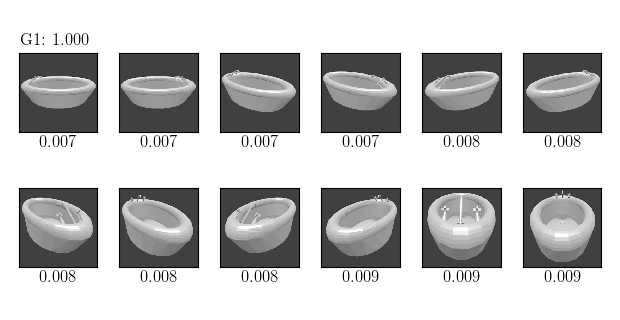
\includegraphics[trim=10 20 10 20, clip]{images/mn-sl-0-3-20/bathtub_0107_0_grouping.png}
		\caption{Blank}
		\label{fig:grouping-0-3-blank}
	\end{subfigure}
	\begin{subfigure}{\textwidth}
		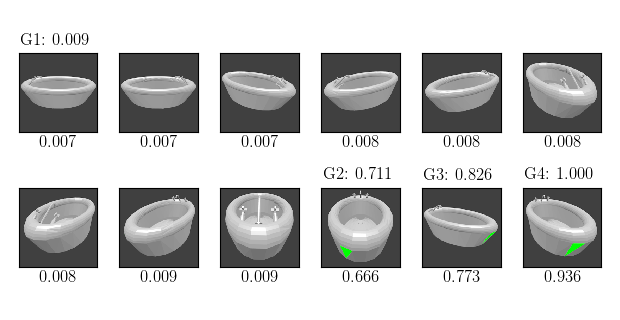
\includegraphics[trim=10 20 10 20, clip]{images/mn-sl-0-3-20/bathtub_0107_1_grouping.png}
		\caption{Green color mark}
		\label{fig:grouping-0-3-green}
	\end{subfigure}
	\begin{subfigure}{\textwidth}
		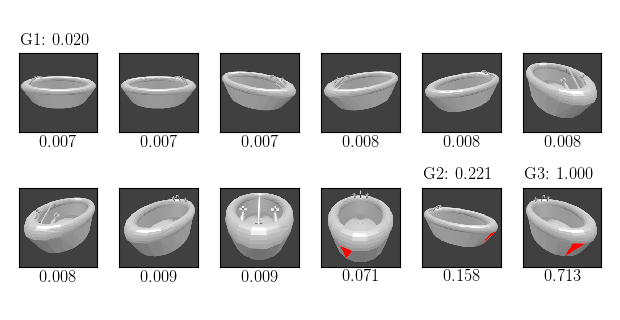
\includegraphics[trim=10 20 10 20, clip]{images/mn-sl-0-3-20/bathtub_0107_2_grouping.png}
		\caption{Red color mark}
		\label{fig:grouping-0-3-red}
	\end{subfigure}
	\caption[Grouping in 0-3 network]{Grouping in 0-3 network. The number below a view is its discrimination score. The one above views is the group weight. All views after a stated group weight are part of this group, until another one is stated.}
	\label{fig:grouping-0-3}
\end{figure}

In \figref{fig:grouping-0-3-blank} a blank object is classified.
Hence, every views are similar discriminative, due to no available colored face.
Thus, the view scores are very similar.
Those little changes presumably depend on a different weight initialization and would be compensated by more training epochs.
Although the scores are very low, the views are fully taken into account because they all belong to the same group with a weight of 1.0.

In this particular case, a normalization of the group weight is not necessary.
Without one the group weight would be $w_g = 0.0079$, thus, decreasing the shape descriptor enormously, but the network would learn that a descriptor close to 0 represents a blank object.
The decision rule would be, if the descriptor represents no color mark, the objects show no color mark.
With the classification of more categories, though, this is not possible anymore, because a very small descriptor cannot just represent any blank object, but the object category class.
If there are two objects, for example, and only one view of each shows a different color mark with a small discrimination score, they would be divided into two groups.
Without a normalization, all views would almost account to the same amount to the shape descriptor.
Hence, the weights in the fully-connected layers for each specific present feature needs to be very large.
With normalization, however, the group with one view is much higher weighted than the not discriminative views.
Hence, normalization removes noise, i.e. not discriminative views, that could influence the prediction unfavorably.

\figref{fig:grouping-0-3-green} and \figref{fig:grouping-0-3-red} show the expected result of a group assignment with color marks.
The views showing the color mark are by far the top-rated views referring to their score.
It looks like, that the grouping module prefers the slightly tilted vertical edge with a color mark to its right for recognizing color marks.
This exact edge is not visible in the first view showing a color mark, due to the change in perspective.
Due to the mesh representation of objects, all color marks are triangles.
It is possible, that the dataset contains more color marks following this shape than in rotated ones, hence, the network focuses on that shape.

Moreover, both figures show exactly the same order.
This shows, that the weights for each color channel are optimized in the same direction.
However, the views with the green color mark are in a closer range regarding the view discrimination score than the ones with the red color mark.
The latter differs extremely.
The least discriminative view containing a color mark is closer to the not discriminative views than the discriminative ones.
It is assumed, that a bad weight initialization caused this problem and a longer training would compensate it.
Nevertheless, the group metric, the group precision for each color class, is at 1.0 for every color mark.
It should be noted, that always only a metric for the non-blank color marks is given.
\begin{figure}
	\centering
	\begin{subfigure}{\textwidth}
		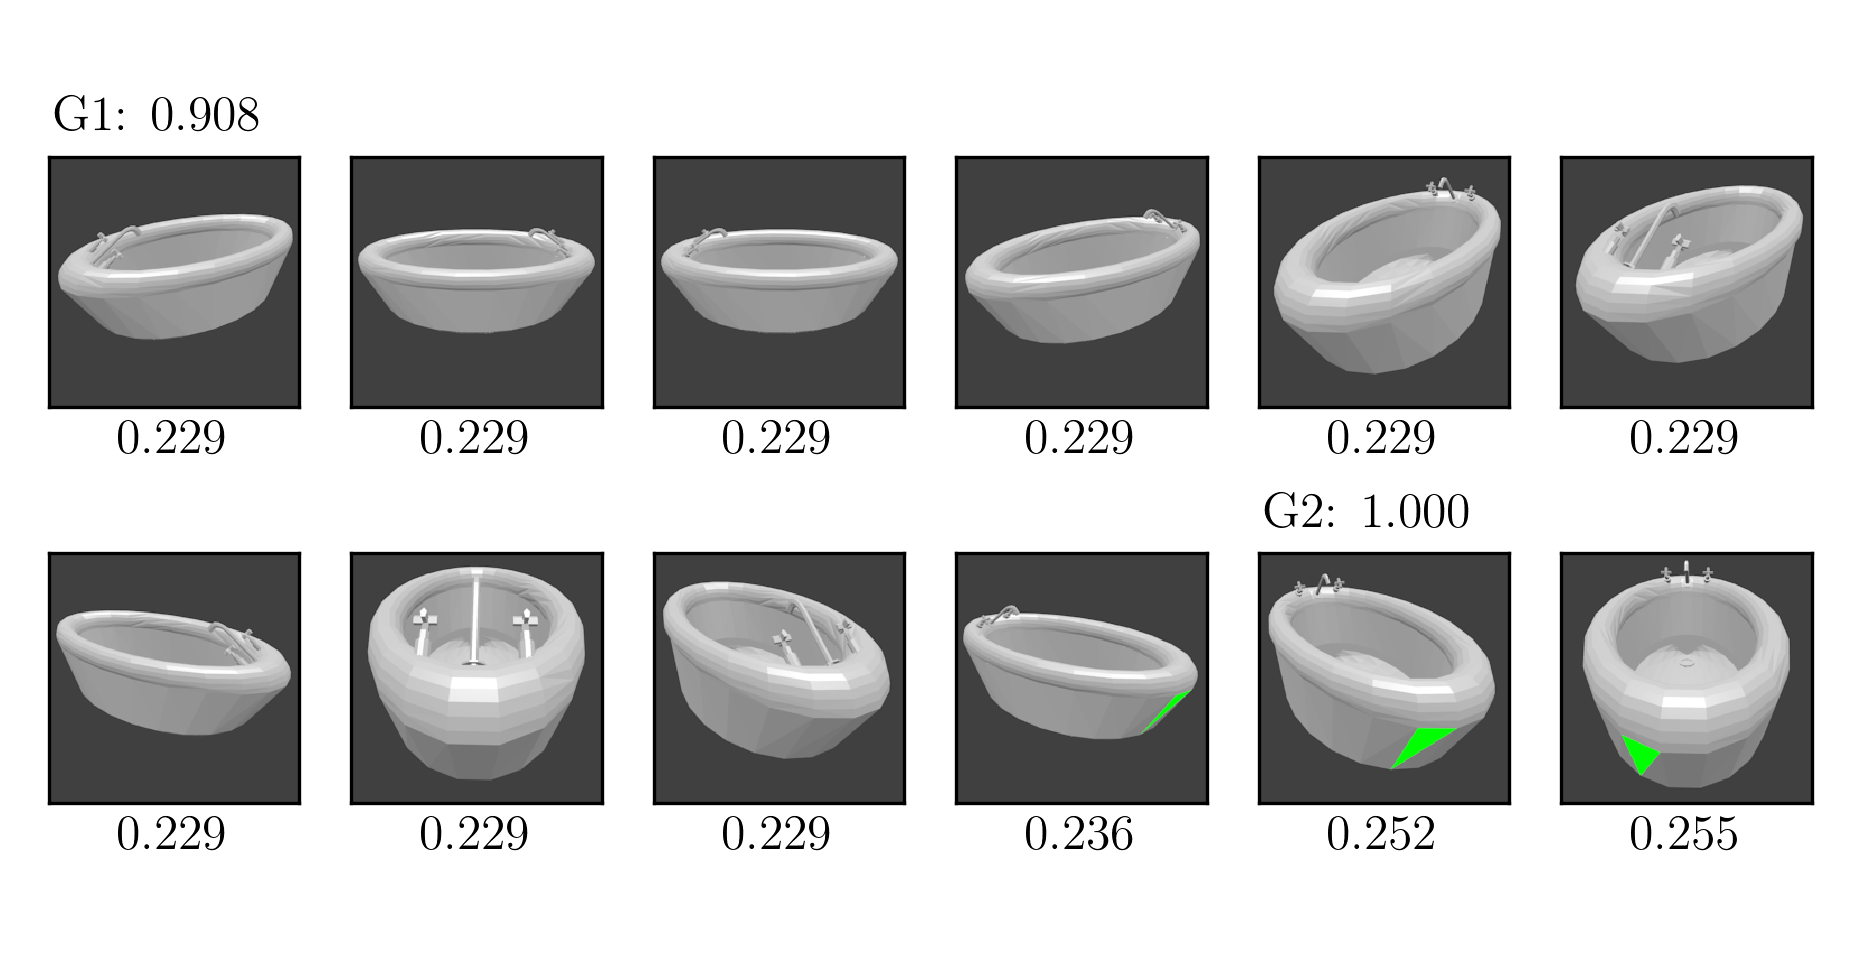
\includegraphics[trim=10 20 10 20, clip]{images/mn-sl-0-4-20/bathtub_0107_1_grouping.png}
		\caption{Green}
		\label{fig:grouping-0-4-green}
	\end{subfigure}
	\begin{subfigure}{\textwidth}
		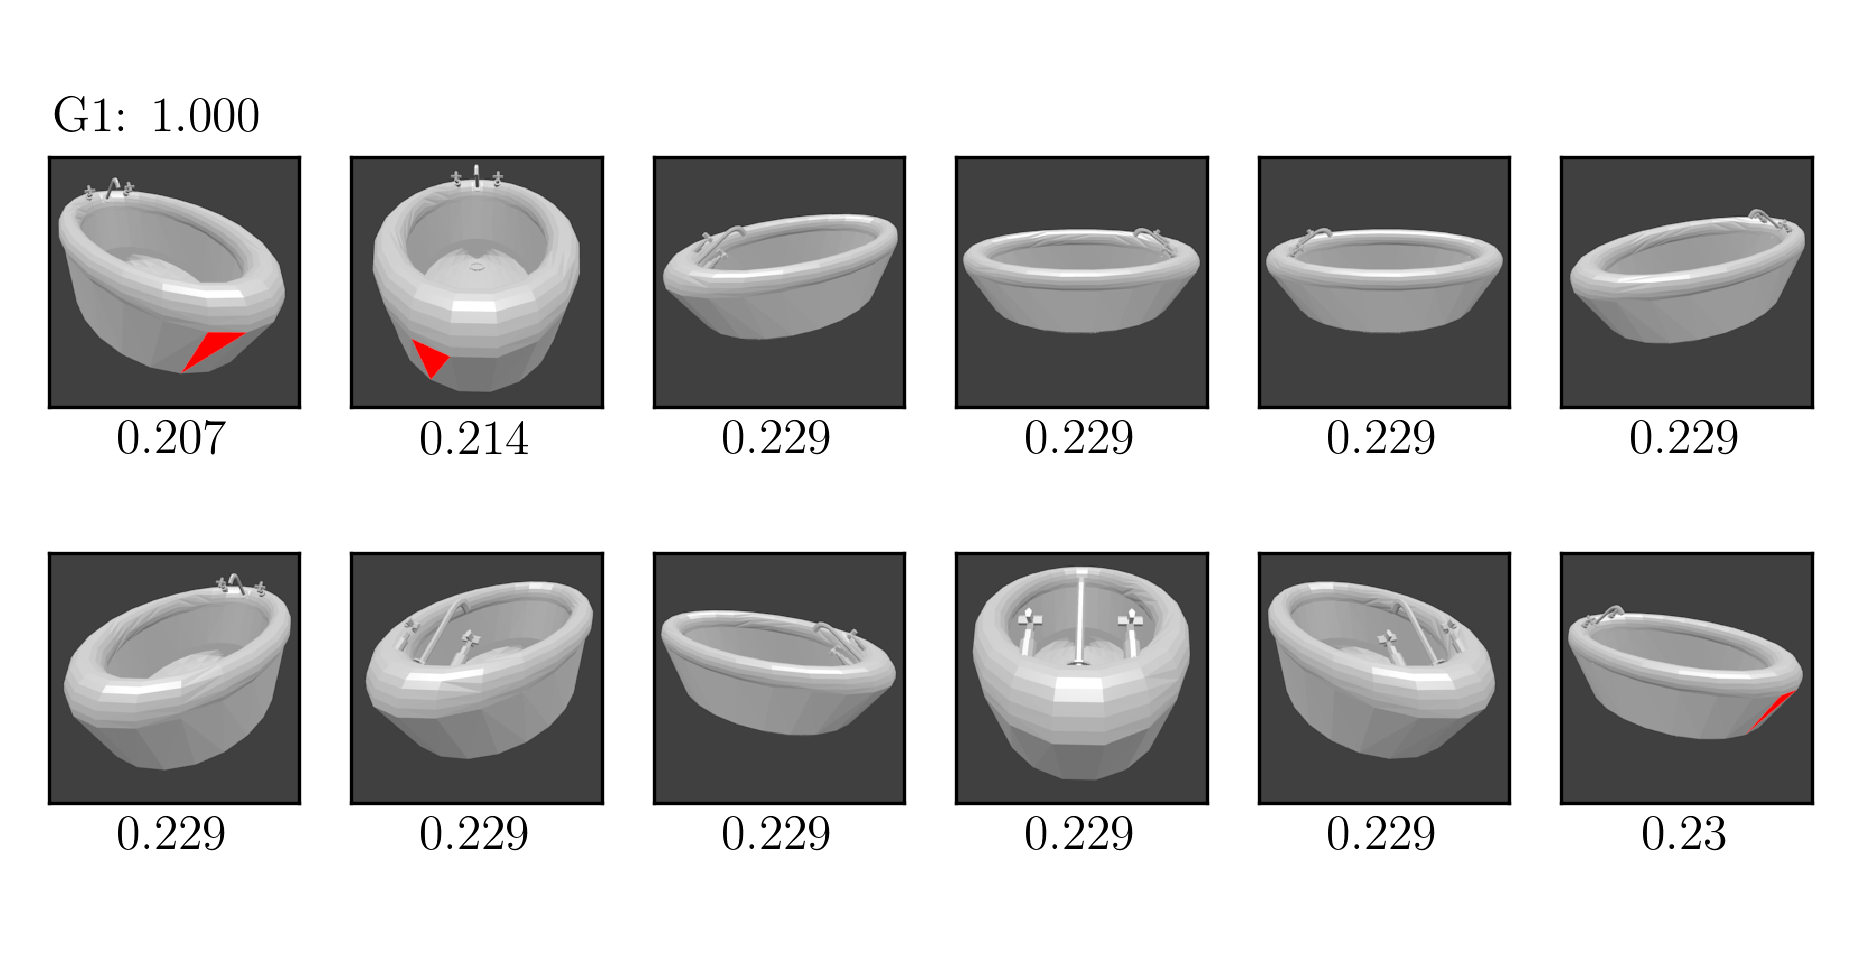
\includegraphics[trim=10 20 10 20, clip]{images/mn-sl-0-4-20/bathtub_0107_2_grouping.png}
		\caption{Red}
		\label{fig:grouping-0-4-red}
	\end{subfigure}
	\begin{subfigure}{\textwidth}
		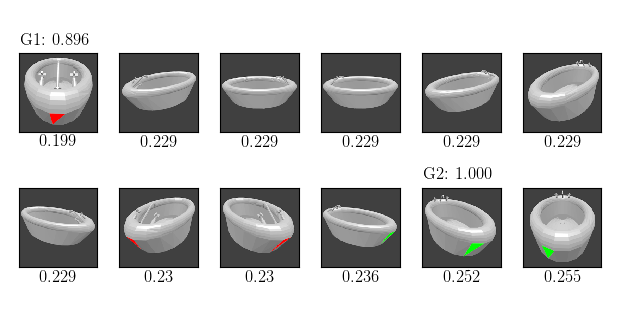
\includegraphics[trim=10 20 10 20, clip]{images/mn-sl-0-4-20/bathtub_0107_3_grouping.png}
		\caption{Green-red}
		\label{fig:grouping-0-4-green-red}
	\end{subfigure}
	\caption[Grouping in 0-4 network]{Grouping in 0-4 network}
	\label{fig:grouping-0-4}
\end{figure}

In \figref{fig:grouping-0-4} the grouping of the 0-4 network is shown, which additionally classifies green-red color marks.
The assignment of the blank object is omitted but all views have a score of 0.229.
This is higher than before and indicating a higher information content.
However, the score is consistent for all blank views in this network.
Compared to the 0-3 network, this network finds different correlations.
This is noticed, because the order of views is different.
Furthermore, not only the views with an available color mark are rated high like in \figref{fig:grouping-0-4-red}, but also the normal views like in \figref{fig:grouping-0-4-green}.
The reason is, that there could be two color marks on a single object.
Hence, a view where a color mark is supposed to be present is rated high, although it is missing.
This means, the discriminative information is the missing color mark, thus, the network uses views to exclude classes for its prediction.
Therefore, a worse group metric than before is expected.
This is reflected by the precision values 0.735, 0.475 and 0.800 for each class.
The averaged precision is 0.670.
This shows that the network focuses most on the green color marks as well because it is more often in the highest weighted group than the red one.
This is also seen in the assignment of the red color mark, where two of three color views are the least discriminative ones.
That suggests, that the red color mark is treated as a sufficient criterion, while the green one is treated as the necessary criterion.
Moreover, it is not surprising, that the green and red color marks are mostly present in the top group.
\begin{figure}
	\centering
	\begin{subfigure}{\textwidth}
		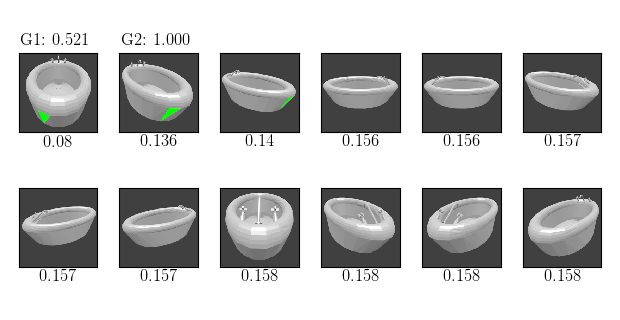
\includegraphics[trim=10 20 10 20, clip]{images/mn-sl-0-5-20/bathtub_0107_1_grouping.png}
		\caption{Green}
		\label{fig:grouping-0-5-green}
	\end{subfigure}
	\begin{subfigure}{\textwidth}
		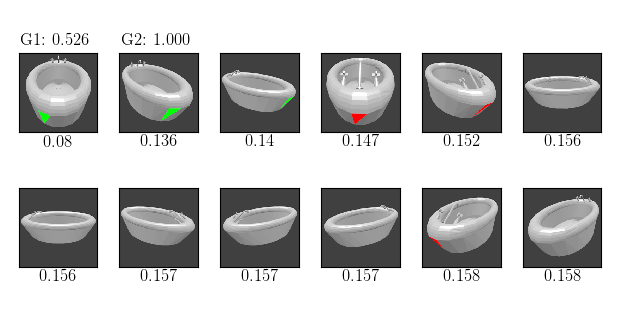
\includegraphics[trim=10 20 10 20, clip]{images/mn-sl-0-5-20/bathtub_0107_3_grouping.png}
		\caption{Green-red}
		\label{fig:grouping-0-5-green-red}
	\end{subfigure}
	\begin{subfigure}{\textwidth}
		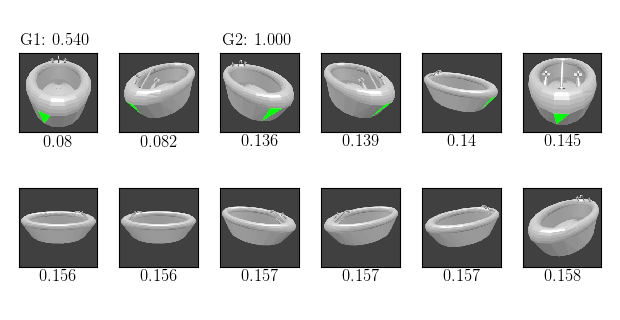
\includegraphics[trim=10 20 10 20, clip]{images/mn-sl-0-5-20/bathtub_0107_4_grouping.png}
		\caption{Green-green}
		\label{fig:grouping-0-5-green-green}
	\end{subfigure}
	\caption[Grouping in 0-5 network]{Grouping in 0-5 network. The number below a view is its discrimination score. The one above views is the group weight. All views after a stated group weight are part of this group, until another one is stated.}
	\label{fig:grouping-0-5}
\end{figure}

The grouping for the 0-5 network is examined, that additionally classifies green-green color marks.
The important results can be seen in \figref{fig:grouping-0-5}.
The group assignment of the blank object is similar to the ones before.
There is only one group and the view discriminative scores are in a range of 0.156 and 0.158.
The group assignment of the red color mark is similar to the one of 0-4.
Though, the second view from earlier changes its position with the top view.
Moreover, the score of every view is decreased by about 0.07.
However, that the highest rated view shows a red color mark is possibly for adding certainty for the classification with avoiding large weights.

For the green color mark, the colored views are the least discriminative ones according to their score.
This is shown in \figref{fig:grouping-0-5-green}.
That effect is necessarily caused by the additional green-green color mark.
An explanation could be, that the network now rates views by missing color marks.
Hence, the shape descriptor becomes smaller the more color marks are available.
This theory is almost supported by the group assignment of green-red, that is shown in \figref{fig:grouping-0-5-green-red}.
Moreover, referring to the view scores, the views showing a green color mark have the exact same score than in the single green case.
However, the theory is adapted, that not the number of color marks is crucial, but rather that every color mark has a range in which it is classified.
Green color marks are less discriminative than red ones and red ones are less discriminative than blank ones.
Using the green-green group assignment from \figref{fig:grouping-0-5-green-green} confirms this more.
The views with a green color mark are less discriminative than the blank ones and also have a lower score than the red ones in the earlier cases.
Thus, the shape descriptor's values are large, if no color mark is visible, neutral if red ones are visible, slightly smaller if green ones are visible, small if both color marks are visible and very small if two green color marks are visible.
For this network, the group metrics are 0.419, 0.469, 0.768, 0.750 with an average of 0.601.
Those of each single color mark and of each double color mark are similar and the average is smaller than in the 0-4 case.
This supports the grouping theory even more in so far, that non-color mark views are mainly members of the top group.
\begin{figure}
	\centering
	\begin{subfigure}{\textwidth}
		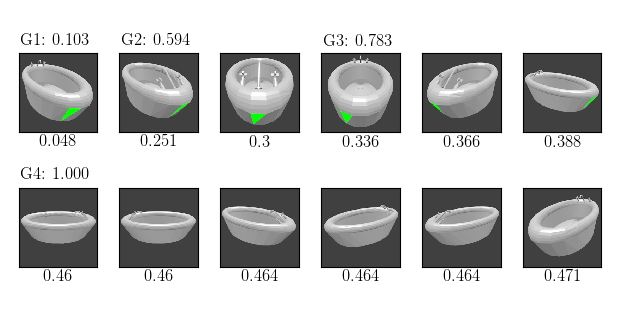
\includegraphics[trim=10 20 10 20, clip]{images/mn-sl-0-6-20/bathtub_0107_4_grouping.png}
		\caption{Green-green}
		\label{fig:grouping-0-6-green-green}
	\end{subfigure}
	\begin{subfigure}{\textwidth}
		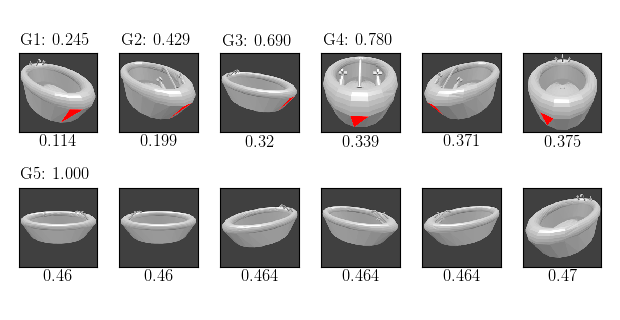
\includegraphics[trim=10 20 10 20, clip]{images/mn-sl-0-6-20/bathtub_0107_5_grouping.png}
		\caption{Red-red}
		\label{fig:grouping-0-6-red-red}
	\end{subfigure}
	\caption[Grouping in 0-6 network]{Grouping in 0-6 network. The number below a view is its discrimination score. The one above views is the group weight. All views after a stated group weight are part of this group, until another one is stated.}
	\label{fig:grouping-0-6}
\end{figure}

To have balanced evaluation results regarding the distribution of color classes, red-red color marks are added, yielding the 0-6 network.
Grouping blank views is almost identical to the earlier cases with the exception of view scores in a range of 0.46 to 0.472.
The order of views for the green color mark has not changed notably.
However, an additional group is created and the scores of the views with a visible color mark changed to 0.336, 0.048 and 0.388.
The remaining scores are in a range of 0.46 to 0.472 which matches the blank case.
In the red color mark case, the most discriminative view from the red color mark prediction of 0-5 is now the third-to-last.
Hence, all views showing color marks are the least discriminative ones with scores of 0.106, 0.313 and 0.358.
The remaining views have identical scores as the other color mark cases.
Moreover, all of those views are assigned to four groups.
In comparison, the green color mark and the red one have similar view scores, where the scores of the blank views are identical.
For the green-red case, all views not showing a color mark are more discriminative than the ones showing one.
This matches almost the grouping in the 0-5 network, but with five groups.
The highest weighted group only contains non-colored views.
Furthermore, the scores of views with a green color mark have the same score than in the single green color mark case.
However, this is applicable to the views with red color marks.
This is due to the fact, that in this case, the second optimal face is colored red, hence, there are no comparable red faces.

For the green-green and red-red case, that are shown in \figref{fig:grouping-0-6}, the group assignment is almost identical.
The first one uses four groups the second five.
Though the view scores are similar, it is noticeable, that compared to each different color mark in the green-red case views with a now green color mark are less discriminative than views with a now red color mark.
Although, both times the general score is higher.
Fortunately, this does not debunk the assumed theory of the group mechanism.
The corresponding group metric scores are 0.217, 0.253, 0.420, 0.381, 0.504 with an average of 0.355.
Their distribution is as expected, but with smaller values than in earlier networks.
This is due to the larger number of groups and the higher diversity of non-colored views to colored views.

For a full understanding of the grouping mechanism, it needs to be examined, if the assumed theory is still valid if additional categories are classified.
Moreover, it is analyzed how the information content of views changes with more category classes, hence, presumably more features the network needs to learn.
This is done in the same order of number of classifications as with only color marks.
First, the 4-0 network is evaluated.
It is supposed, that similar views like opposite perspectives of a symmetrical object are assigned into the same group because they contain similar features.
For example, the views of the left and right side of a car look almost identical, due to having the same contours but in a mirrored direction.
\begin{figure}
	\centering
	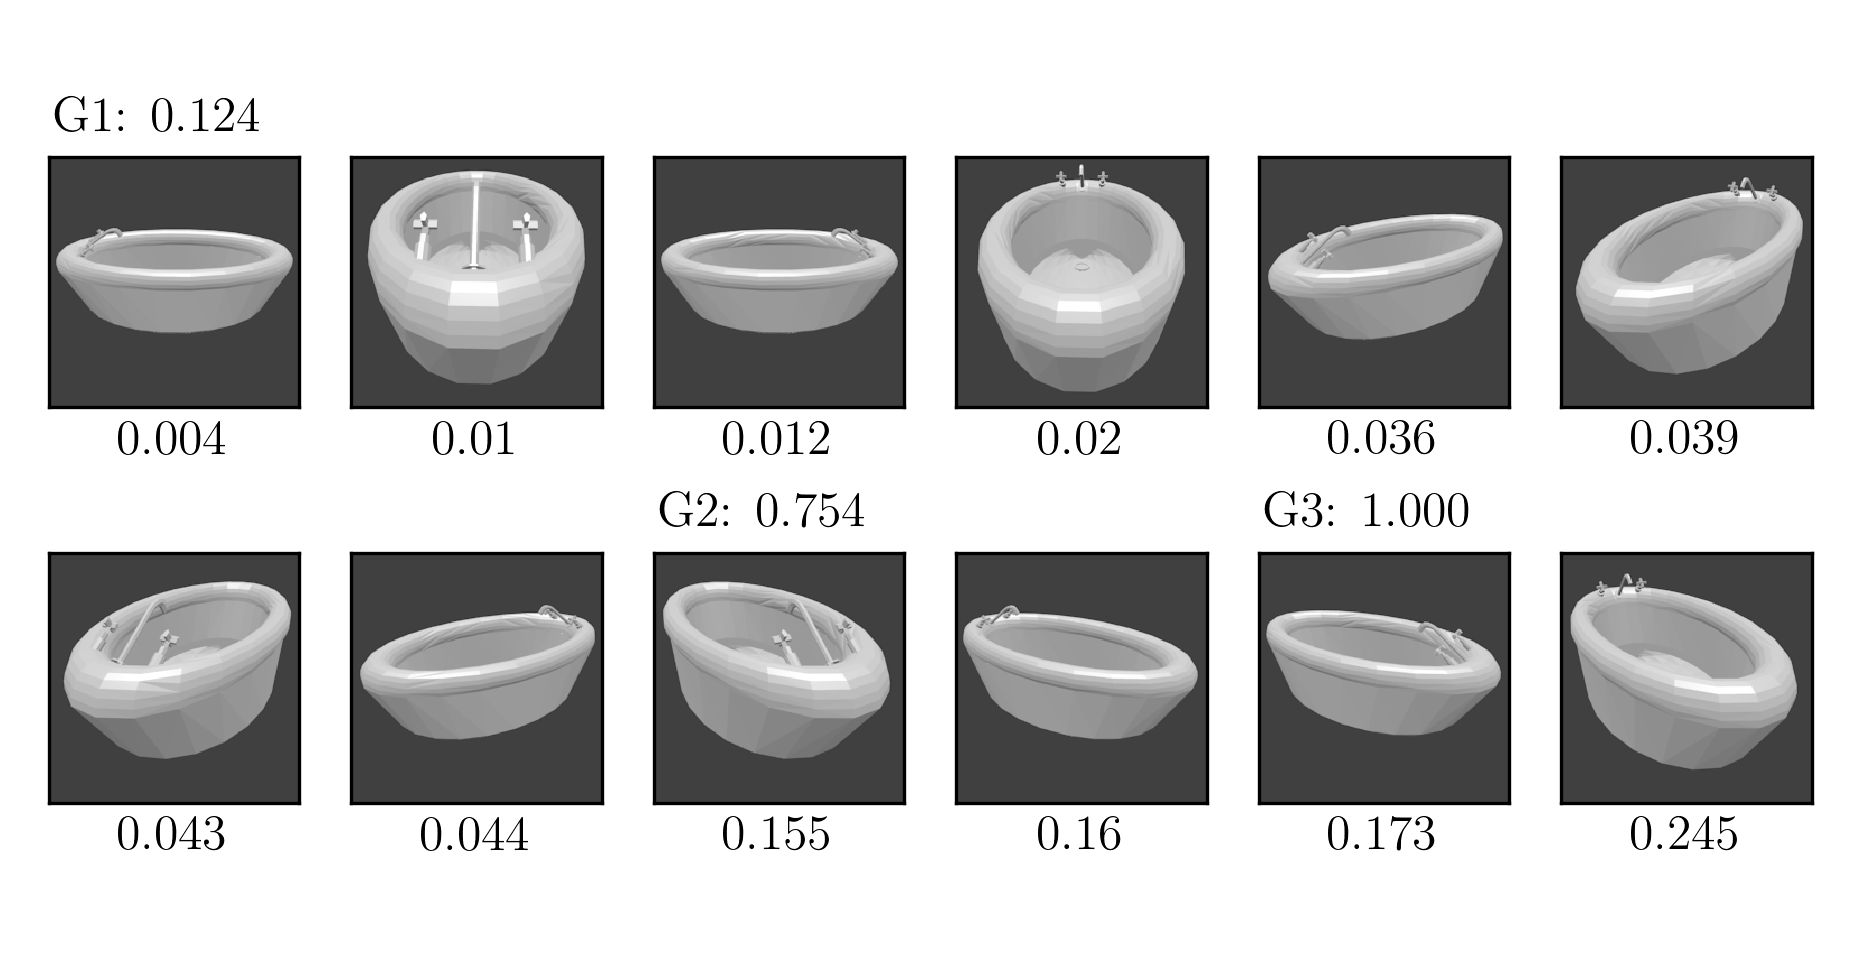
\includegraphics[trim=10 20 10 20, clip]{images/mn-sl-4-0-20/bathtub_0107_0_grouping.png}
	\caption[Grouping in 4-0 network]{Grouping in 4-0 network. The number below a view is its discrimination score. The one above views is the group weight. All views after a stated group weight are part of this group, until another one is stated.}
	\label{fig:grouping-4-0}
\end{figure}
A group assignment is shown in \figref{fig:grouping-4-0}.
It can be seen that the assumption is wrong.
Instead, the network prefers objects or features, respectively, that are diagonal from top left to bottom right.
This is validated by more multi-view predictions of different objects.
That such preferences are learned is already assumed from the 0-3 grouping and is obviously applicable to networks with more classes, in particular, category ones.
The scores, however, are difficult to interpret.
For doing this it is necessary to compare all weights and activations, without achieving a real benefit, because the functionality of the grouping algorithm is already validated by using only color marks.

The grouping for the remaining networks is briefly summarized.
Their assignments are shown in \figref{fig:grouping-4-3}, \figref{fig:grouping-4-4}, \figref{fig:grouping-4-5} and \figref{fig:grouping-4-6}.
\begin{figure}
	\centering
	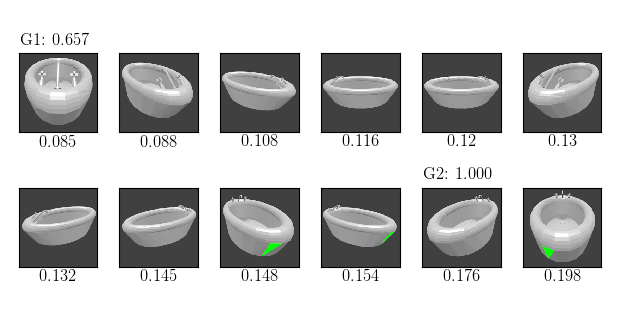
\includegraphics[trim=10 20 10 20, clip]{images/mn-sl-4-3-20/bathtub_0107_1_grouping.png}
	\caption[Grouping in 4-3 network]{Grouping in 4-3 network. The number below a view is its discrimination score. The one above views is the group weight. All views after a stated group weight are part of this group, until another one is stated.}
	\label{fig:grouping-4-3}
\end{figure}
\begin{figure}
	\centering
	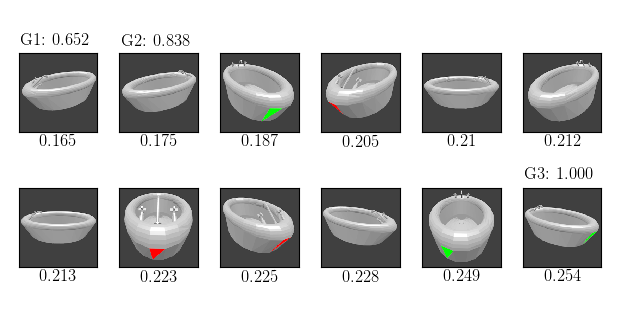
\includegraphics[trim=10 20 10 20, clip]{images/mn-sl-4-4-20/bathtub_0107_3_grouping.png}
	\caption[Grouping in 4-4 network]{Grouping in 4-4 network. The number below a view is its discrimination score. The one above views is the group weight. All views after a stated group weight are part of this group, until another one is stated.}
	\label{fig:grouping-4-4}
\end{figure}
\begin{figure}
	\centering
	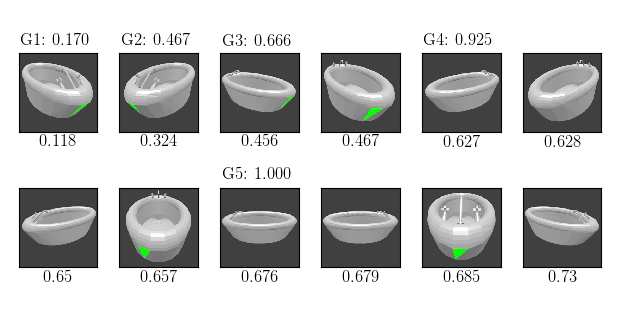
\includegraphics[trim=10 20 10 20, clip]{images/mn-sl-4-5-20/bathtub_0107_4_grouping.png}
	\caption[Grouping in 4-5 network]{Grouping in 4-5 network. The number below a view is its discrimination score. The one above views is the group weight. All views after a stated group weight are part of this group, until another one is stated.}
	\label{fig:grouping-4-5}
\end{figure}
\begin{figure}
	\centering
	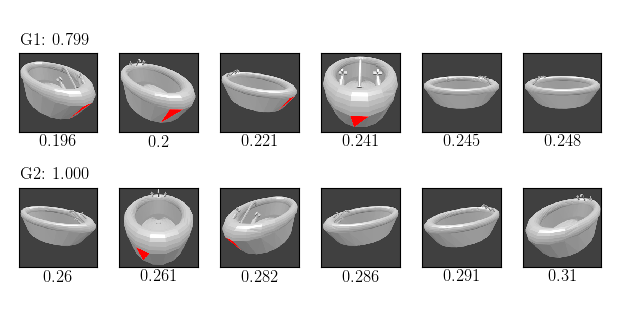
\includegraphics[trim=10 20 10 20, clip]{images/mn-sl-4-6-20/bathtub_0107_5_grouping.png}
	\caption[Grouping in 4-6 network]{Grouping in 4-6 network. The number below a view is its discrimination score. The one above views is the group weight. All views after a stated group weight are part of this group, until another one is stated.}
	\label{fig:grouping-4-6}
\end{figure}
It can be seen, that each top group always contains at least one view with a visible color mark.
Furthermore, the remaining ones are not necessarily discriminative, because depending on the number of color marks it is more important to find features classifying the category.
Moreover, the more classes exist, the more groups are created.
That suggests, that the assumption from before, that the values of shape descriptors of different classes are in different ranges, could be valid, because this way the network is more flexible in weighting views or view descriptors, respectively.